% !TEX root = ../ausarbeitung.tex
%Unter Evaluation der Result Teil mit "nackten Zahlen" als Boxplot + Textuell %Mittelwert und Standardabweichung. Wenn möglich noch ein statistischen Test %zwischen den einzelnen Kategorien.
\chapter{Results} %TODO Ref
In diesem Kapitel werden die Ergebnisse des Nutzertests präsentiert. Die Darstellung erfolgt nach den Kategorien, die durch den GEQ definiert wurden. Anhand von Boxplots werden die Ergebnisse der jeweiligen Kategorie von der ThirdPerson Ansicht und der TopDown Ansicht gegenüber gestellt.
Zunächst wird ein Gesamtbild der beiden Perspektiven, für einen groben Überblick, gegenüber gestellt.
%TODO Bilder neu machen mit geringerer Höhe 
\begin{figure}[h!tb]
	\centering
	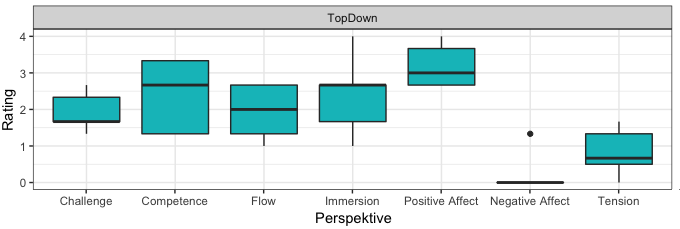
\includegraphics[width=0.65\textwidth]{topDownPlot}
	\caption{Boxplots der TopDown Perspektive\label{fig:topdownbox}}
\end{figure}
\begin{figure}[h!tb]
	\centering
	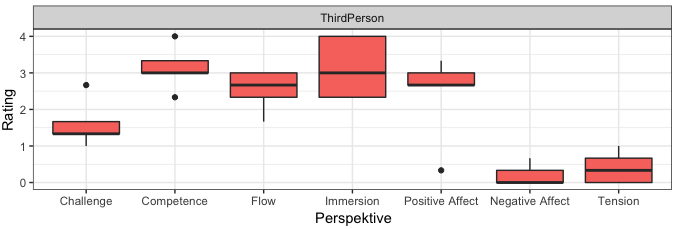
\includegraphics[width=0.65\textwidth]{thirdPersonPlot}
	\caption{Boxplots der ThirdPerson Perspektive\label{fig:thirdpersonbox}}
\end{figure}


\section{Challenge}
\begin{figure}[h!tb]
	\centering
	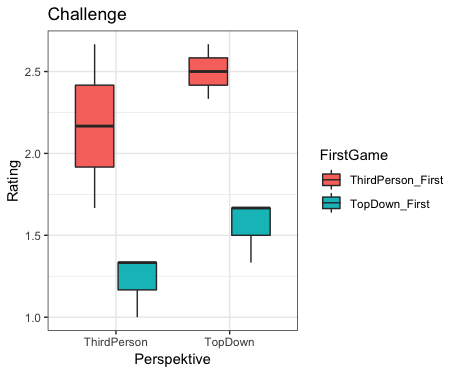
\includegraphics[width=0.65\textwidth]{challengePlot}
	\caption{Boxplot der Kategorie Challenge\label{fig:challengebox}}
\end{figure}
Der Durchschnitt in der Challenge Kategorie beträgt für TopDown  $1.93\overline{3}(SD = 0.55)$ und für die ThirdPerson-Variante $1.6(SD =0.64 )$
\section{Competence}
\begin{figure}[h!tb]
	\centering
	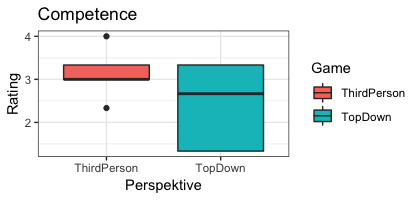
\includegraphics[width=0.65\textwidth]{competencePlot}
	\caption{Boxplot der Kategorie Competence\label{fig:competencebox}}
\end{figure}
Der Durchschnitt in der Competence Kategorie beträgt für TopDown  $2.4(SD = 1.01)$ und für die ThirdPerson-Variante $3.1\overline{3}(SD =0.61 )$
\section{Flow}
\begin{figure}[h!tb]
	\centering
	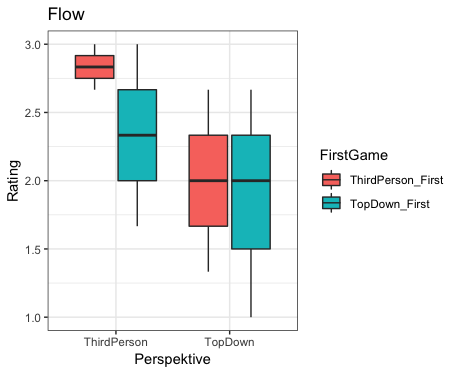
\includegraphics[width=0.65\textwidth]{flowPlot}
	\caption{Boxplot der Kategorie Flow\label{fig:flowbox}}
\end{figure}
Der Durchschnitt in der Flow Kategorie beträgt für TopDown  $1.9\overline{3}(SD = 0.76)$ und für die ThirdPerson-Variante $2.5\overline{3}(SD =0.56 )$
\section{Immersion}
\begin{figure}[h!tb]
	\centering
	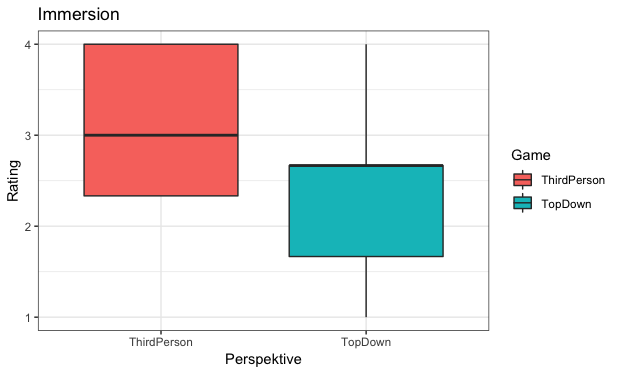
\includegraphics[width=0.65\textwidth]{immersionPlot}
	\caption{Boxplot der Kategorie Immersion\label{fig:immersionbox}}
\end{figure}
Der Durchschnitt in der Immersion Kategorie beträgt für TopDown  $2.4(SD = 1.14)$ und für die ThirdPerson-Variante $3.1\overline{3}(SD =0.84 )$
\section{Negative Effect}
\begin{figure}[h!tb]
	\centering
	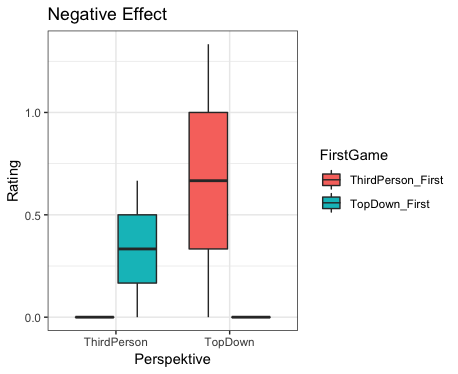
\includegraphics[width=0.65\textwidth]{negEffPlot}
	\caption{Boxplot der Kategorie Negative Effect\label{fig:negeffbox}}
\end{figure}
Der Durchschnitt in der Negative Effect Kategorie beträgt für TopDown  $0.2\overline{6}(SD = 0.6)$ und für die ThirdPerson-Variante $0.2(SD =0.3 )$
\section{Positive Effect}
\begin{figure}[htb]
	\centering
	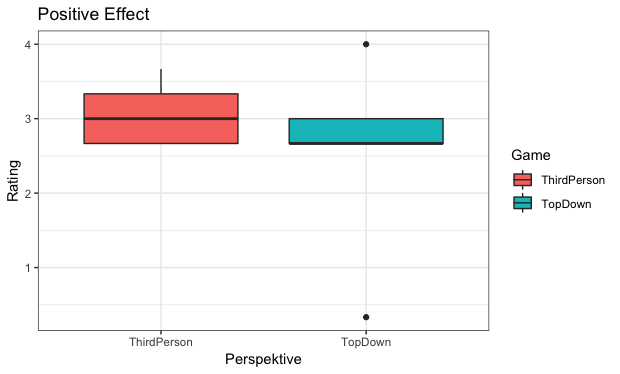
\includegraphics[width=0.65\textwidth]{posEffPlot}
	\caption{Boxplot der Kategorie Positive Effect\label{fig:poseffbox}}
\end{figure}
Der Durchschnitt in der Positive Effect Kategorie beträgt für TopDown  $2.5\overline{3}(SD = 1.35)$ und für die ThirdPerson-Variante $3.0\overline{6}(SD =0.43 )$
\section{Tension}
\begin{figure}[htb]
	\centering
	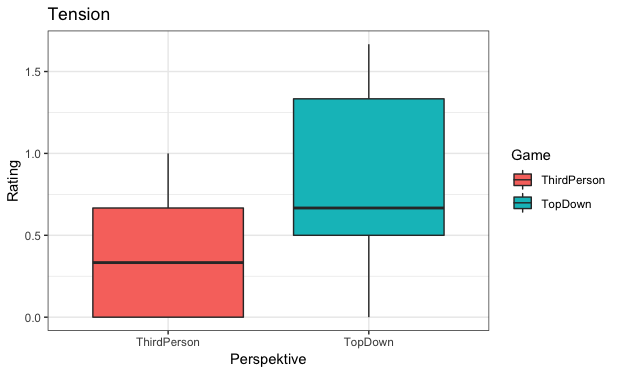
\includegraphics[width=0.65\textwidth]{tensionPlot}
	\caption{Boxplot der Kategorie Tension\label{fig:tensionbox}}
\end{figure}
Der Durchschnitt in der Tension Kategorie beträgt für TopDown  $0.8\overline{3}(SD = 0.67)$ und für die ThirdPerson-Variante $0.4(SD =0.43 )$
\section{Schriftliche Fragen}
\subsection{Welches Spiel hat dir mehr Spaß gemacht?}
Diese Frage wurde im Nutzertest von allen Nutzern mit der ThirdPerson Variante beantwortet. Angegebene Gründe waren:
\begin{itemize}
\item man war näher dran und die Zahlen waren größer
\item 3D wurde als schöner empfunden
\item durch die nähere Perspektive hatte man eher das Gefühl teil des Spiels zu sein.
\end{itemize}
\subsection{Welches Spiel fandest du schwieriger?}
Hier wurde von fast allen Nutzern die TopDown Perspektive angegeben. Begründungen waren wie folgt notiert:
\begin{itemize}
\item da es das erste Spiel war und man dadurch die Steuerung noch nicht im Griff hatte
\item Durch die Perspektive war alles zu klein und dadurch zu schwer
\end{itemize}
Eine Person hat hier ebenfalls die ThirdPerson Perspektive angegeben mit der Begründung, dass Äpfel, die auf den Kopf der Schlange herunterfallen, direkt als gegessen gelten.
\subsection{Hattest du Probleme dich im Spiel zurecht zu finden?}
Diese Frage wurde sehr unterschiedlich beantwortet. Zwei der Nutzer hatten keine Probleme bei beiden Versionen. Jeweils ein Nutzer hatte Probleme mit der ThirdPerson Perspektive und einer mit der TopDown Perspektive. Der letzte Nutzer des Tests hat nichts angegeben.
\hfil\rule{0.4\textwidth}{0.4pt}